\section{Experimental Evaluation}\label{sec:experiments}
\subsection{Scenario, baselines, and protocol}
Table~\ref{tab:parameters} gives the common scenario and training parameters.
Device positions are sampled uniformly by area in a disk; gains are
$g_i=10^{-4}\max(d_i/1\,\mathrm{m},1)^{-4}$. Positions and phases remain fixed
within an episode. The three traffic classes have equal offered load per
device, so increasing $N$ raises load without changing its per-device average.
The class counts for $N=4,6,8,12$ are respectively $(2,1,1)$, $(2,2,2)$,
$(3,3,2)$, and $(4,4,4)$.

\begin{table}[t]
\caption{Scenario and learning parameters.}\label{tab:parameters}
\centering\footnotesize
\begin{tabular}{ll}
\toprule
Parameter & Value \\
\midrule
Devices / subchannels & $N\in\{4,6,8,12\}$ / $K=4$ \\
Slot duration / bandwidth & 1 ms / 1 MHz per subchannel \\
Cell radius / path-loss exponent & 100 m / 4 \\
Noise density / noise figure & $-174$ dBm/Hz / 7 dB \\
Positive transmit powers & 5, 10, 15, 19, 23 dBm \\
Periods $P_i$ (slots) & 10, 20, 40 \\
Packet sizes $L_i$ (bits) & 6144, 12\,288, 24\,576 \\
Per-device violation allowance & $\epsilon=0.05$ \\
Evaluation horizon / warm-up & 2000 / 200 slots \\
Training episode / rollout & 600 / 128 slots \\
Parallel environments / epochs & 16 / 4 PPO epochs \\
Actor GRU / critic hidden widths & 64 / 256, 256 \\
Actor / critic learning rates & $3\!\times\!10^{-4}$ / $10^{-3}$ \\
Discount / GAE parameter & 0.99 / 0.95 \\
PPO clip / gradient norm limit & 0.2 / 0.5 \\
Training budget per seed & $20\!\times\!10^6$ environment slots \\
\bottomrule
\end{tabular}
\end{table}

We train a separate shared policy for each $N$, using seeds 101, 202, and 303.
Each episode draws a topology--phase instance uniformly from a pool of one
million training instances. Training, development, validation, and test pools
are disjoint. Actor and critic parameters are not shared across network sizes;
the study tests generalization to new instances at a trained $N$, rather than
zero-shot transfer to a new $N$. The entropy coefficient decreases linearly
from 0.01 to zero over the first ten million slots. Total training slots are
summed over the 16 environments. Minibatches contain four environment
trajectories. The penalty and dual step size were selected in an initial
two-million-slot study at $N=8$ and transferred to all long runs.

Four local rules provide non-learning comparisons. \emph{Random-max} selects
a random subchannel and maximum power whenever a packet is pending.
\emph{Sticky-max} retains its preceding subchannel if its previous service
meets the current required pace, and otherwise reselects randomly, always at
maximum power. \emph{Lazy-pacing} selects power from its latest link estimate
to meet $s_i/D_i$, changing subchannel when necessary.
The strongest evaluated feasible rule, \emph{paced-sticky}, remembers its
gain across packets, retains a subchannel within 3 dB of the least-interfered
one, and otherwise switches with probability 0.5 to a subchannel within
3 dB of the minimum. It chooses the lowest power predicted to serve
$(1+m)s_i/D_i$ bits, probing at maximum power before its gain is known.
Its margin $m$ is calibrated over
$\{0,0.1,0.25,0.5,1,2,4,8,16,32\}$ separately for each $N$, selecting
$0,0.25,0.5,8$, respectively. Thus it is an energy-aware, load-calibrated
comparison rather than only a maximum-power random-access rule.

Validation uses 64 instances and one stochastic execution per instance,
approximately every million training slots. An episode is feasible if every
device has empirical violation rate at most 0.05. With $M_i$ evaluated
packets and $V_i$ violations, this is exactly
$V_i\le\lfloor0.05M_i\rfloor$ for all $i$. We denote the fraction of
feasible episodes by $F$. Among checkpoints with validation $F\ge0.95$, we
select the smallest mean normalized energy; if none qualifies, we select
the highest $F$, breaking ties by energy. MAPPO-D jointly selects its
initial multiplier. The selected and final checkpoints are both evaluated.

Testing uses 200 held-out instances per $N$, two executions per instance,
and all three training seeds. Random execution uses independent private
device streams with common seed assignments across methods. Evaluated packets
have deadlines in $(200,2000]$; their complete transmit energy, including
energy spent on failed packets, defines $E$. This packet-set accounting matches
the centralized denominators. Separately, reported mean power counts all
transmissions in slots $[200,2000)$. Methods satisfy the empirical protocol
criterion when their aggregate $F\ge0.95$. This threshold uses the point
estimate, not the lower confidence limit. Energy superiority is judged only
between methods satisfying it. We use 10\,000 two-level bootstrap resamples
over training seeds and instances, averaging repetitions within an instance.
Differences resample instances jointly and training seeds independently
between methods. All intervals are 95\% percentile intervals.

\subsection{Held-out energy and reliability}
\begin{figure*}[t]
\centering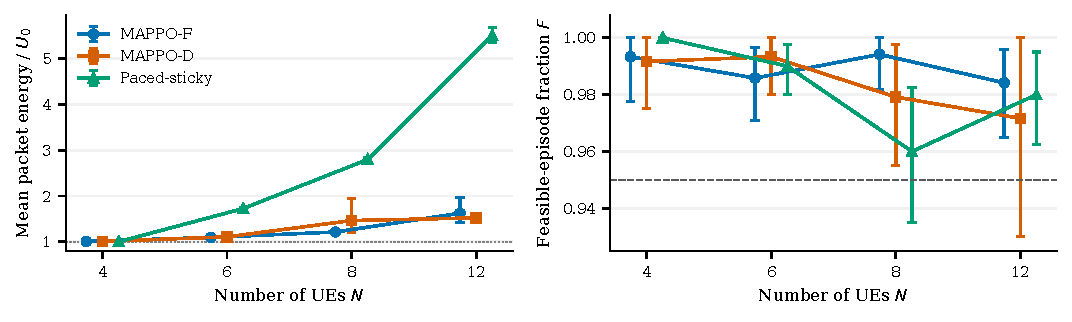
\includegraphics[width=\textwidth]{figures/test_performance.pdf}
\caption{Held-out test performance of selected checkpoints. The energy
denominator $U_0$ is a feasible centralized zero-loss schedule; it equals
the zero-loss optimum for $N=4$. Bars show two-level 95\% bootstrap intervals.
The dashed line at $F=0.95$ is the empirical protocol threshold.}
\label{fig:test}
\end{figure*}

\begin{table}[t]
\caption{All distributed methods on the held-out test set. Each cell is
$F$ / mean $E/U_0$. $\dagger$ denotes failure of the $F\ge0.95$ criterion;
its energy is descriptive only.}
\label{tab:all}
\centering\scriptsize\setlength{\tabcolsep}{2.2pt}
\begin{tabular}{lcccc}
\toprule
Method & $N=4$ & $N=6$ & $N=8$ & $N=12$ \\
\midrule
MAPPO-F & 0.993/1.01 & 0.986/1.09 & 0.994/1.21 & 0.984/1.62 \\
MAPPO-D & 0.992/1.01 & 0.993/1.11 & 0.979/1.46 & 0.972/1.52 \\
Paced-sticky & 1.000/1.00 & 0.990/1.73 & 0.960/2.80 & 0.980/5.51 \\
Random-max & 1.000/9.87 & 1.000/9.32 & 1.000/9.34 & 0.995/8.93 \\
Sticky-max & 1.000/10.36 & 1.000/10.05 & 1.000/10.40 & 0.983/10.21 \\
Lazy-pacing & 0.797/5.34$^\dagger$ & 0.657/4.98$^\dagger$ & 0.287/5.76$^\dagger$ & 0.000/8.02$^\dagger$ \\
\bottomrule
\end{tabular}

\end{table}

Figure~\ref{fig:test} and Table~\ref{tab:all} show that MAPPO-F satisfies the
empirical feasibility criterion at all four loads. For $N=6,8,12$, its mean
$E/U_0$ is \EnergySix, \EnergyEight, and \EnergyTwelve, compared with
1.725, 2.798, and 5.508 for paced-sticky. The reductions are
\SavingSix\%, \SavingEight\%, and \SavingTwelve\%, computed as one minus
the ratio of the two methods' mean normalized energies. They are not means
of per-instance percentage reductions. The paired differences
(MAPPO-F minus paced-sticky) have intervals
$[-0.659,-0.603]$, $[-1.632,-1.541]$, and $[-4.179,-3.535]$, respectively;
all exclude zero. Corresponding mean transmit powers are
\PowerSix, \PowerEight, and \PowerTwelve\,mW/device, versus
6.83, 12.07, and 29.24\,mW/device for paced-sticky.

At $N=4$, paced-sticky attains the exact zero-loss reference. MAPPO-F has
$E/U_0=1.007$ with interval $[1.004,1.010]$, and $F=0.993$.
This is a useful reference-recovery check, with no improvement over the local
rule at this load. At higher loads the learned policy's advantage over the
local rules grows, yet its distance from centralized scheduling also grows.
MAPPO-F's mean $E/L_0$ is 1.119, 1.349, and 2.289 for $N=6,8,12$.
At $N=12$, energy remains 62.3\% above the feasible orthogonal reference.
These ratios show substantial remaining room for improvement, with the
zero-loss qualification of Section~\ref{sec:bounds}.

Maximum-power rules retain high feasibility but consume approximately
9--10 times the centralized reference energy. Lazy-pacing fails the
feasibility criterion at every load, reaching $F=0$ at $N=12$.
Thus lowering power using only a recent pacing estimate does not by itself
resolve multiuser interference. The calibrated paced-sticky rule is
substantially stronger and remains the main energy comparison.

\subsection{Does local dual adaptation improve performance?}
Both selected MAPPO variants satisfy the empirical criterion at every $N$.
However, the paired energy difference between MAPPO-F and MAPPO-D has a
95\% interval containing zero at every load. At $N=8$, their means are
1.213 and 1.463, but the difference interval is $[-0.737,0.005]$;
at $N=12$, the means are 1.623 and 1.522, with interval
$[-0.119,0.452]$. One less effective training seed strongly affects each
comparison. These results give no statistically resolved energy advantage
to either constraint treatment; they do not establish equivalence.

Checkpoint dependence provides a practical distinction. MAPPO-F's final
checkpoints remain feasible at all four loads, with $F$ between 0.987 and
0.992. MAPPO-D's final $F$ falls to 0.915 and 0.938 at $N=8$ and 12.
The fixed-penalty variant therefore provides the simpler empirical reference
for this study. A separate short-budget global-multiplier variant selected
its untrained initial checkpoint and achieved test $F=0.592$ at $N=8$.
That result concerns this training configuration and selection outcome;
it does not show that global primal--dual methods generally fail.

\subsection{Training and observed coordination}
\begin{figure*}[t]
\centering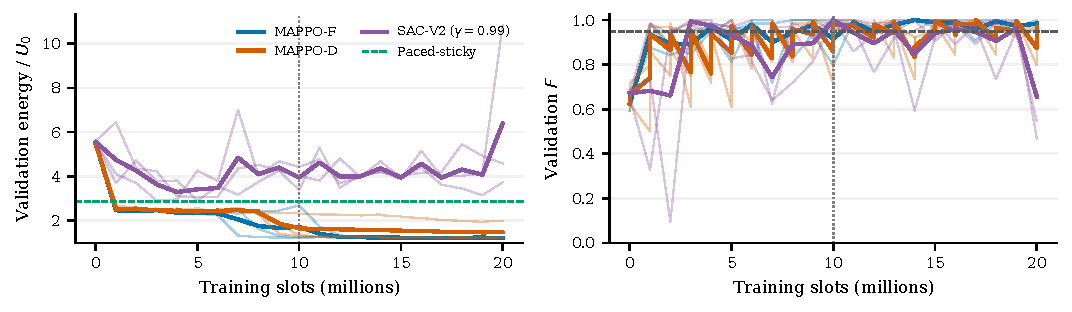
\includegraphics[width=\textwidth]{figures/learning_n8.pdf}
\caption{Validation trajectories for $N=8$. Thin lines show the three
training seeds; thick lines show their means, without smoothing. The vertical
dotted line marks the end of entropy annealing at ten million slots. For
MAPPO-D, curves use the validation-selected initialization at each checkpoint.
These are training diagnostics, not additional test-set evaluations.}
\label{fig:learning}
\end{figure*}

The gain requires substantial training. Figure~\ref{fig:learning} shows a
large energy decrease between roughly six and twelve million slots.
The separately trained two-million-slot MAPPO-F configuration has test
$E/U_0=2.321$ and $F=0.989$ at $N=8$; the long configuration reaches 1.213
and 0.994. Budget and entropy schedule both change between these configurations,
so the difference cannot be attributed to either change alone.

\begin{figure}[t]
\centering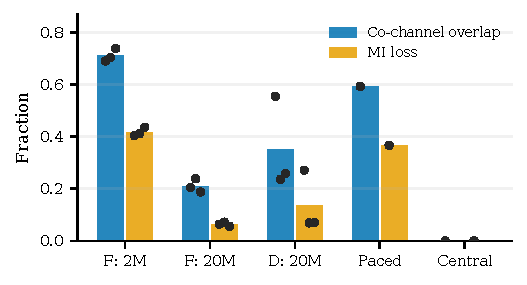
\includegraphics[width=\columnwidth]{figures/coordination_n8.pdf}
\caption{Descriptive validation diagnostics at $N=8$: short (2M) and long
(20M) training configurations. F and D denote MAPPO-F and MAPPO-D.
Bars are means across seeds; dots are individual seed summaries. The
central reference and paced-sticky have one summary each.}
\label{fig:coordination}
\end{figure}

To examine behavior, we replay selected policies on the validation set.
Co-channel overlap is the fraction of transmissions sharing their subchannel
with another active device; it does not mean automatic packet loss in the
SINR model. Interference loss is one minus the ratio of total actual mutual
information to the interference-free mutual information of those same
transmissions at the same powers. For MAPPO-F, the short-budget configuration
has mean overlap 0.712 and loss 0.418; the long configuration reduces these
to approximately 0.211 and 0.064 (Fig.~\ref{fig:coordination}).
Paced-sticky has overlap 0.594 and loss 0.367. Long-trained MAPPO-F also
uses the 5 and 10 dBm levels for about 83\% of transmissions.
Its probability of transmitting conditional on having a pending packet
is 0.61--0.76 across seeds, versus 1 for paced-sticky, consistent with using
silence while work is pending. This conditional fraction is not the fraction
of all device--slots that are occupied.

Together these observations support an association between energy savings,
lower-power transmission, and less harmful overlap. They do not isolate the
causal contributions of recurrence, power adaptation, or silence. A separate
validation-only short-budget experiment appended interference and own-action
features at lags of 10, 20, and 40 slots. It changed MAPPO-F's mean $E/U_0$
from 2.337 to 2.432, and MAPPO-D's from 2.404 to 2.385; neither met the
predeclared 5\% improvement threshold. This negative result is limited to
the tested features and budget, not all ways of exploiting periodicity.

\subsection{Reliability tails and scope}
The aggregate feasibility criterion allows a small set of bad episodes.
In a post hoc analysis pooling both learned variants over all four loads,
128 of 9600 executions are infeasible. In 108 of these, the worst device is
75--100 m from the AP, and in 83 its period is 40 slots. Such a device has
45 evaluated packets and can miss only two before the episode becomes
infeasible. Some failures are severe: an $N=4$ MAPPO-F execution contains
a device violation rate of 0.733. Average feasibility must therefore not be
read as a uniform reliability guarantee or a URLLC claim.

Three training seeds limit precision about optimization variability, and
the tested channel and feedback are idealized. Accounting for feedback,
circuit, and processing energy could change the benefit of spreading
transmissions. Further, this completed evaluation contains no independently
implemented literature-based learning comparator; it establishes an advantage
over the evaluated local rules. An information-matched XR-SBPC-style SAC
comparison is outside the completed evidence reported here.
